% ============================================================
% Beamer — ISLP Lecture Series — IMPROVED EDITION
% Advanced Module A10: Causal Inference from Observational Data
% ============================================================
\documentclass[aspectratio=169,11pt]{beamer}
\usepackage[utf8]{inputenc}\usepackage[T1]{fontenc}\usepackage[english]{babel}
\usepackage{graphicx}\usepackage{booktabs}\usepackage{amsmath,amssymb,amsfonts}
\usepackage{mathtools}\usepackage{hyperref}\usepackage{xcolor}
\usepackage{verbatim}\usepackage{alltt}
\usepackage{tikz}\usetikzlibrary{calc,arrows.meta,positioning,shapes}
\usepackage{tcolorbox}\tcbuselibrary{skins}

\usetheme{Madrid}\usecolortheme{default}
\setbeamertemplate{navigation symbols}{}
\setbeamertemplate{footline}[frame number]
\setbeamertemplate{blocks}[rounded][shadow=false]
\setbeamertemplate{headline}{%
  \leavevmode\hbox{%
    \begin{beamercolorbox}[wd=\paperwidth,ht=2.2ex,dp=0.9ex]{section in head/foot}%
      {\fontsize{4.6}{5.2}\selectfont%
       \insertsectionnavigationhorizontal{\paperwidth}{}{\hskip0pt plus1filll}}%
    \end{beamercolorbox}}%
}
\setbeamerfont{section in head/foot}{size=\tiny}
\setbeamerfont{palette primary}{size=\tiny}
\setbeamerfont{palette tertiary}{size=\tiny}
\setbeamerfont{section in toc}{size=\footnotesize}

\usepackage{listings}
\definecolor{pyKw}{RGB}{0,0,180}\definecolor{pyStr}{RGB}{20,120,40}
\definecolor{pyCom}{RGB}{120,120,120}\definecolor{accent}{RGB}{38,70,140}
\lstdefinestyle{Pystyle}{language=Python,basicstyle=\ttfamily\footnotesize,
  keywordstyle=\color{pyKw}\bfseries,commentstyle=\color{pyCom}\itshape,
  stringstyle=\color{pyStr},showstringspaces=false,upquote=true,
  columns=fullflexible,breaklines=true,literate={~}{{$\sim$}}1}
\lstset{style=Pystyle}

% Tighter TOC spacing (place AFTER \lstset, BEFORE \AtBeginSection)
\usepackage{etoolbox}
\makeatletter
\patchcmd{\beamer@sectionintoc}{\vskip1.5em}{\vskip.6em}{\typeout{TOCPATCH-OK}}{\typeout{TOCPATCH-FAIL}}
\makeatother

\AtBeginSection[]{\begin{frame}{Outline}\footnotesize
  \tableofcontents[currentsection,sectionstyle=show/shaded,subsectionstyle=show/show/hide]
\end{frame}}

\newcommand{\islpsource}[1]{%
  \vfill\hfill{\tiny\itshape\color{gray}Source: #1 \textemdash{} ISLP, James et al.\ (2023).}\par
}

\newtcolorbox{takeaway}[1][Takeaway]{enhanced,colback=green!4,colframe=green!50!black,
  boxrule=0pt,leftrule=2.5pt,arc=2pt,fonttitle=\bfseries,title=#1,
  left=2mm,right=2mm,top=1mm,bottom=1mm}
\newtcolorbox{numexample}[1][Worked example]{enhanced,colback=orange!4,colframe=orange!70!black,
  boxrule=0pt,leftrule=2.5pt,arc=2pt,fonttitle=\bfseries,title=#1,
  left=2mm,right=2mm,top=1mm,bottom=1mm}
\newtcolorbox{readme}[1][How to read this]{enhanced,colback=blue!4,colframe=accent,
  boxrule=0pt,leftrule=2.5pt,arc=2pt,fonttitle=\bfseries,title=#1,
  left=2mm,right=2mm,top=1mm,bottom=1mm}

\title{Quantitative Research Methods}
\subtitle{Causal Inference from Observational Data\\[2pt]{\small Advanced module A10 --- optional self-study}}
\author{Prof.\ Dr.\ Christoph Weisser}
\date{}\graphicspath{{images/}}

\newtcolorbox{exercise}[1][Exercise]{enhanced, fontupper=\footnotesize, colback=purple!4, colframe=purple!55!black, boxrule=0pt, leftrule=2.5pt, arc=2pt, fonttitle=\bfseries, title=#1, left=2mm, right=2mm, top=1mm, bottom=1mm}
\newtcolorbox{solutionbox}[1][Solution]{enhanced, colback=teal!5, colframe=teal!55!black, boxrule=0pt, leftrule=2.5pt, arc=2pt, fonttitle=\bfseries, title=#1, left=2mm, right=2mm, top=1mm, bottom=1mm}
\newtcolorbox{longexercise}[1][Extended exercise (15 min)]{enhanced, fontupper=\footnotesize, colback=violet!6, colframe=violet!55!black, boxrule=0pt, leftrule=3pt, arc=2pt, fonttitle=\bfseries, title=#1, left=2mm, right=2mm, top=1mm, bottom=1mm}

% Reclaim ~2pt of body height (custom nav headline makes full slides tip over by ~1.83pt)
\addtobeamertemplate{frametitle}{}{\vspace{-2pt}}

\newtcolorbox{labnote}[1][Run this live in the lab notebook]{enhanced, fontupper=\footnotesize, colback=cyan!7, colframe=cyan!45!black, boxrule=0pt, leftrule=3pt, arc=2pt, fonttitle=\bfseries, title=#1, left=2mm, right=2mm, top=1mm, bottom=1mm}

% Common-mistake callout --- crimson, for the error to pre-empt
\newtcolorbox{mistake}[1][Common mistake]{enhanced, fontupper=\footnotesize, colback=red!4, colframe=red!60!black, boxrule=0pt, leftrule=3pt, arc=2pt, fonttitle=\bfseries, title=#1, left=2mm, right=2mm, top=1mm, bottom=1mm}

\begin{document}
\begin{frame}[plain]\titlepage\end{frame}

\begin{frame}{Where this module fits}
  \footnotesize
  \begin{center}
  \begin{tabular}{@{}p{3.9cm}p{8.4cm}@{}}
    \toprule
    \textbf{Course chapter / module} & \textbf{What this module builds on it} \\
    \midrule
    Ch.\ 3 --- linear regression & Adjustment \emph{is} multiple regression; omitted-variable bias \\
    Ch.\ 4 --- logistic regression & The propensity score is a fitted logistic model \\
    Ch.\ 5 --- resampling & Seeded simulations that know the true effect \\
    Module A1 --- RCTs & Potential outcomes, selection bias --- assumed throughout \\
    \bottomrule
  \end{tabular}
  \end{center}
  \vspace{2pt}
  \begin{takeaway}[The question A1 left open]
    Module A1 ended with the one clean design: randomise, then compare. This module
    asks what you can still learn when \textbf{nobody randomised} --- the data are
    observational, treatment was \emph{chosen}, and every naive comparison is a
    mixture of effect and selection.
  \end{takeaway}
  {\scriptsize One of twelve optional advanced modules; self-study. Every number on
  these slides is reproduced by \texttt{make\_figures.py} in the module folder.}
\end{frame}

\begin{frame}{Contents}\small\tableofcontents[hideallsubsections]
  \vfill
  {\tiny Optional and advanced material is collected in the \textbf{appendix} at the end of the deck.}
\end{frame}

\begin{frame}{Notation in this module}
  \footnotesize
  \begin{center}
  \begin{tabular}{@{}ll@{}}
    \toprule
    \textbf{Symbol} & \textbf{Meaning} \\
    \midrule
    $D \in \{0,1\}$ & treatment received (not assigned --- nobody assigned it) \\
    $Y(1), Y(0)$ & potential outcomes with and without treatment (module A1) \\
    $U$ & a confounder: causes both $D$ and $Y$ \\
    $X$ & observed covariates (possibly a noisy proxy for $U$) \\
    $e(x) = \Pr(D=1 \mid X=x)$ & the propensity score \\
    $Z$ & an instrument: shifts $D$, touches $Y$ only through $D$ \\
    $\tau$ & the causal effect we are after (ATT/ATE) \\
    $\delta$ & auxiliary-regression coefficient of $D$ on the confounder \\
    \bottomrule
  \end{tabular}
  \end{center}
\end{frame}

\begin{frame}{Sources and references}
  \begin{block}{Primary textbook}
    James, Witten, Hastie, Tibshirani \& Taylor (2023),
    \emph{An Introduction to Statistical Learning, with Applications in Python},
    Springer. --- The regression and classification machinery this module reuses.
  \end{block}
  \begin{block}{Canonical further reading (optional)}
    Angrist \& Pischke, \emph{Mostly Harmless Econometrics} (2009);
    Hern\'an \& Robins, \emph{Causal Inference: What If} (2020) --- both develop
    everything here at full depth.
  \end{block}
\end{frame}

\begin{frame}{Learning objectives}
  By the end of this module you will be able to:
  \begin{itemize}
    \item \textbf{Explain} why a naive group comparison in observational data mixes
          the causal effect with selection bias.
    \item \textbf{Derive} the omitted-variable-bias formula and predict the sign and
          size of the bias.
    \item \textbf{Adjust} for observed confounders by regression, stratification and
          propensity-score matching --- and say what adjustment can never fix.
    \item \textbf{Apply} difference-in-differences to a two-group, two-period table
          and state the parallel-trends assumption.
    \item \textbf{Use} an instrumental variable via the Wald estimator, and check the
          three conditions an instrument must satisfy.
  \end{itemize}
\end{frame}

\begin{frame}{Roadmap of this module}
  \begin{takeaway}[From ``the data say'' to ``the design says'']
    \begin{enumerate}
      \item The problem: selection, confounding, and one running simulation.
      \item Omitted-variable bias: the formula behind every headline gone wrong.
      \item Adjustment: regression, stratification, propensity-score matching.
      \item Difference-in-differences: using time as the control.
      \item Instrumental variables: borrowing someone else's randomness.
      \item Python lab, summary, appendix.
    \end{enumerate}
  \end{takeaway}
\end{frame}

% ============================================================
\section{The Problem}
% ============================================================

\begin{frame}{The running example: a job-training programme}
  \footnotesize
  A firm offers a voluntary training programme. Ability $U$ drives both
  \textbf{who signs up} ($D$) and \textbf{later earnings} ($Y$):
  $Y = 2 + \smash{\underbrace{1.0}_{\text{true effect}}} \cdot D + 1.5\,U + \varepsilon$,
  \; $D = \mathbf{1}\{0.9\,U + \eta > 0\}$, \; $n = 2000$.
  \par\smallskip
  \begin{center}
    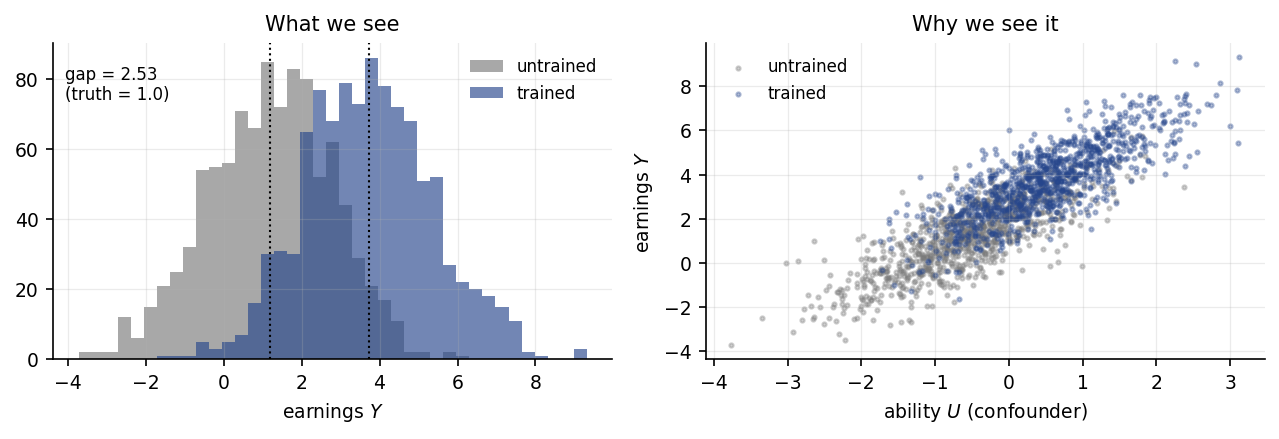
\includegraphics[width=0.86\textwidth,height=0.42\textheight,keepaspectratio]{cha10_confounding.png}
  \end{center}
  \begin{takeaway}[The gap is not the effect]
    The naive difference in means is $\mathbf{2.53}$; the true effect is
    $\mathbf{1.0}$. The right panel shows why: the trained were more able
    \emph{before} training.
  \end{takeaway}
\end{frame}

\begin{frame}{Confounder, mediator, collider --- three roles, one picture}
  \begin{center}
  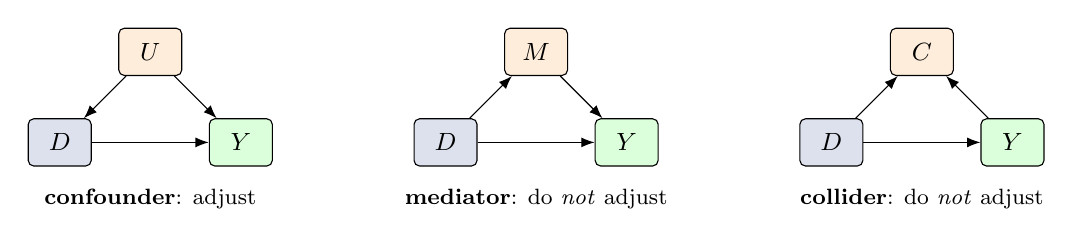
\begin{tikzpicture}[font=\small,
      box/.style={draw, rounded corners=2pt, minimum width=8mm, minimum height=6mm}]
    \foreach \cx/\top/\lab/\mode in {0/$U$/{\textbf{confounder}: adjust}/conf,
                                       4.9/$M$/{\textbf{mediator}: do \emph{not} adjust}/med,
                                       9.8/$C$/{\textbf{collider}: do \emph{not} adjust}/col} {
      \node[box, fill=orange!14] (T-\mode) at (\cx, 1.15) {\top};
      \node[box, fill=accent!16] (D-\mode) at (\cx - 1.15, 0) {$D$};
      \node[box, fill=green!14]  (Y-\mode) at (\cx + 1.15, 0) {$Y$};
      \draw[-{Latex}] (D-\mode) -- (Y-\mode);
      \node[below=1.5mm of {\cx, -0.32}, font=\footnotesize] {\lab};
    }
    \draw[-{Latex}] (T-conf) -- (D-conf); \draw[-{Latex}] (T-conf) -- (Y-conf);
    \draw[-{Latex}] (D-med) -- (T-med);   \draw[-{Latex}] (T-med) -- (Y-med);
    \draw[-{Latex}] (D-col) -- (T-col);   \draw[-{Latex}] (Y-col) -- (T-col);
  \end{tikzpicture}
  \end{center}
  \begin{readme}[How to read this]
    \footnotesize
    Arrows are causes. A \textbf{confounder} sits \emph{upstream} of both $D$ and $Y$
    and must be adjusted away. A \textbf{mediator} carries the effect --- adjusting
    for it deletes the very thing you measure. A \textbf{collider} is caused by both
    --- adjusting for it \emph{creates} spurious association. So ``control for
    everything'' is not a strategy: what to adjust for is a \emph{causal} decision,
    made from the diagram, not from $p$-values.
  \end{readme}
\end{frame}

\begin{frame}{Exercise A10.1 --- Adjust, or leave alone? [Concept]}
  \begin{exercise}
    You study the effect of \textbf{smoking} ($D$) on \textbf{heart disease} ($Y$).
    For each variable, say whether adjusting for it helps, is harmless, or actively
    biases the estimate --- and name its role:
    \begin{enumerate}
      \item \textbf{Age} --- older people smoke more (in this cohort) and have more
            heart disease.
      \item \textbf{Tar deposits in the lungs} --- caused by smoking; contribute to
            disease.
      \item \textbf{Hospitalisation} --- both heavy smokers and heart patients are
            over-represented in a sample recruited \emph{at a hospital}.
    \end{enumerate}
  \end{exercise}
\end{frame}

\begin{frame}{Solution --- Exercise A10.1}
  \begin{solutionbox}
    \footnotesize
    \textbf{Method.} Place each variable in the diagram relative to $D$ and $Y$;
    the position decides.
    \begin{enumerate}
      \item \textbf{Age: confounder} ($\text{Age} \to D$, $\text{Age} \to Y$).
            Adjust --- without it the smoking effect absorbs the age effect.
      \item \textbf{Tar: mediator} ($D \to \text{Tar} \to Y$). Do \emph{not} adjust:
            comparing smokers and non-smokers \emph{at the same tar level} removes
            the pathway through which smoking does its damage, biasing the total
            effect toward zero.
      \item \textbf{Hospitalisation: collider} ($D \to H \leftarrow Y$). Recruiting
            only hospital patients \emph{conditions} on $H$ and manufactures a
            (typically negative) spurious association --- smokers in hospital are
            there partly \emph{because} they smoke, patients without heart disease
            partly because of other illness.
    \end{enumerate}
  \end{solutionbox}
  \begin{mistake}
    Adding every available covariate to the regression ``to be safe''. Item 2 and
    item 3 are both cases where more adjustment gives a \emph{worse} answer.
  \end{mistake}
\end{frame}

% ============================================================
\section{Omitted-Variable Bias}
% ============================================================

\begin{frame}{The omitted-variable-bias formula}
  Suppose the truth is the \textbf{long} regression, but you fit the \textbf{short} one:
  \[
    \text{long: } Y = \beta_0 + \tau D + \gamma U + \varepsilon
    \qquad\qquad
    \text{short: } Y = b_0 + b_D\, D + e
  \]
  \begin{block}{Rule}
    \[
      \boxed{\; b_D \;=\; \tau + \gamma\,\delta \;}
      \qquad\text{where } U = \delta_0 + \delta D + v
      \text{ (the auxiliary regression).}
    \]
  \end{block}
  \begin{readme}[How to read this]
    The bias is a \emph{product}: how strongly the omitted variable drives the
    outcome ($\gamma$) $\times$ how different the groups are on it ($\delta$).
    Either factor zero $\Rightarrow$ no bias. Both positive $\Rightarrow$ you
    \emph{overstate} the effect.
  \end{readme}
  {\scriptsize\itshape Chapter 3 showed coefficients move when predictors enter;
  this formula says by exactly how much --- for variables you cannot even observe.}
\end{frame}

\begin{frame}{The bias is linear in the confounder's strength}
  \begin{center}
    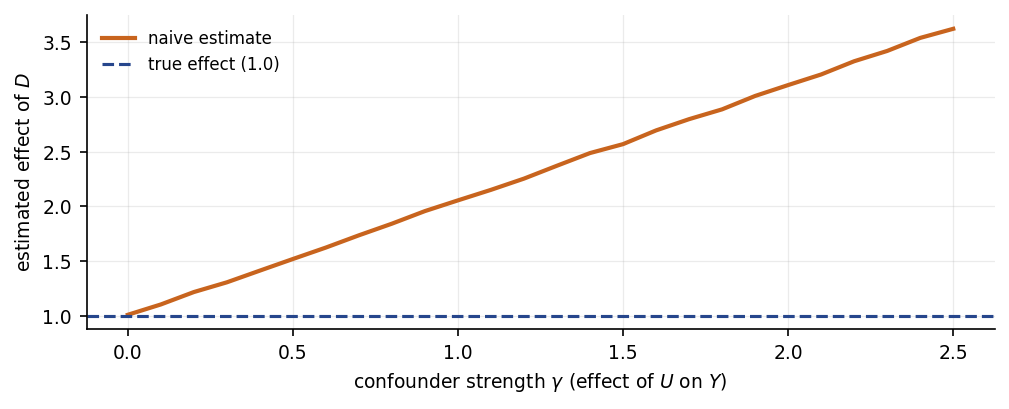
\includegraphics[width=0.78\textwidth,height=0.46\textheight,keepaspectratio]{cha10_ovb.png}
  \end{center}
  \begin{takeaway}[Read off the simulation]
    \footnotesize
    Dialling the confounder's effect $\gamma$ from $0$ to $2.5$, the naive estimate
    climbs linearly with slope $\approx 1.05$ --- which \emph{is} $\delta$, the
    ability gap between the self-selected groups. At $\gamma = 1.5$:
    $1.0 + 1.5 \times 1.05 \approx 2.5$, the naive gap we saw.
  \end{takeaway}
\end{frame}

\begin{frame}{Exercise A10.2 --- Sign and size the bias [Math]}
  \begin{exercise}
    A study of \textbf{private tutoring} ($D$) on \textbf{exam scores} ($Y$, points)
    omits \textbf{parental income} $U$ (in \$10k). Assume the long model
    $Y = \beta_0 + \tau D + \gamma U + \varepsilon$ with $\tau = 5$, $\gamma = 1.5$,
    and the auxiliary regression $U = \delta_0 + \delta D + v$ with $\delta = 0.8$.
    \begin{enumerate}
      \item What does the short regression of $Y$ on $D$ estimate?
      \item A second omitted variable, \textbf{prior struggle}, has $\gamma = -2$
            and $\delta = 1.2$ (struggling students get tutors). Its bias?
      \item With \emph{both} omitted, can you sign the total bias without a computer?
    \end{enumerate}
  \end{exercise}
\end{frame}

\begin{frame}{Solution --- Exercise A10.2}
  \begin{solutionbox}
    \footnotesize
    \textbf{Method.} Apply $b_D = \tau + \sum_j \gamma_j \delta_j$, one omitted
    variable at a time; biases from independent confounders add.
    \begin{enumerate}
      \item $b_D = 5 + 1.5 \times 0.8 = 5 + 1.2 = \mathbf{6.2}$ --- tutoring looks
            $24\%$ better than it is, because richer families buy more of it.
      \item Bias $= \gamma\delta = (-2)(1.2) = \mathbf{-2.4}$ --- struggling students
            select \emph{into} tutoring, dragging the tutored group's scores down.
      \item Total: $5 + 1.2 - 2.4 = \mathbf{3.8}$. The two selections push in
            \emph{opposite} directions, and here the negative one wins --- naive
            comparisons can just as easily \emph{understate} an effect.
    \end{enumerate}
    \textbf{Take-away.} You rarely know $\gamma$ and $\delta$; the formula's real use
    is a \emph{sensitivity argument}: ``how strong would a confounder have to be to
    explain my estimate away?''
  \end{solutionbox}
\end{frame}

% ============================================================
\section{Adjustment \& Matching}
% ============================================================

\begin{frame}{Strategy 1: regression adjustment --- and its honest limit}
  \begin{block}{Rule}
    If \textbf{all} confounders are observed as $X$ (\emph{unconfoundedness}),
    regressing $Y$ on $D$ \emph{and} $X$ recovers the effect:
    $\;\hat\tau = $ coefficient of $D$ in $Y \sim D + X$.
  \end{block}
  \begin{numexample}[{{The running simulation, adjusted}}]
    We observe only a noisy proxy $X = U + \text{noise}$. Adjusting for it moves the
    estimate from the naive $\mathbf{2.53}$ to $\mathbf{1.35}$ --- much closer to the
    truth $1.0$, but \emph{not there}: the noise in the proxy leaves residual
    confounding behind.
  \end{numexample}
  \begin{takeaway}[The assumption does all the work]
    Adjustment removes exactly the bias carried by \textbf{what you measured}. The
    claim ``no unmeasured confounders'' is not testable from the data --- it is an
    argument you must make about the world.
  \end{takeaway}
\end{frame}

\begin{frame}{Strategy 2: stratify --- compare like with like}
  \begin{readme}[The idea in one sentence]
    Cut the data into groups (strata) inside which $X$ is essentially constant,
    compare treated and control \emph{within} each stratum, then average the
    within-stratum gaps.
  \end{readme}
  \begin{numexample}[Why it works]
    Within a stratum, treated and control have the same $X$ --- so the $\gamma\delta$
    term of the bias formula is switched off (for the measured $X$). The naive
    comparison is a \emph{single} stratum: everyone at once.
  \end{numexample}
  \begin{takeaway}[Simpson's warning]
    The within-stratum gaps and the pooled gap can even have \emph{opposite signs}
    --- module A1's Simpson slide is exactly this phenomenon. Stratification is the
    cure, when the strata are confounders.
  \end{takeaway}
\end{frame}

\begin{frame}{Exercise A10.3 --- Stratification by hand [Math]}
  \begin{exercise}
    A voluntary coaching programme; $X \in \{\text{low}, \text{high}\}$ prior skill.
    Mean outcomes (group sizes in parentheses):
    \begin{center}
    \footnotesize
    \begin{tabular}{@{}lcc@{}}
      \toprule
      & \textbf{coached} & \textbf{not coached} \\
      \midrule
      low skill  & $5.0$ \;($n=20$) & $4.0$ \;($n=80$) \\
      high skill & $9.0$ \;($n=80$) & $8.0$ \;($n=20$) \\
      \bottomrule
    \end{tabular}
    \end{center}
    \begin{enumerate}
      \item Compute the naive difference in means (pool the strata).
      \item Compute the stratified estimate (average the within-stratum gaps,
            weighting each stratum by its total size).
      \item Explain the gap between the two numbers in one sentence.
    \end{enumerate}
  \end{exercise}
\end{frame}

\begin{frame}{Solution --- Exercise A10.3}
  \begin{solutionbox}
    \footnotesize
    \textbf{Method.} Naive $=$ overall treated mean $-$ overall control mean;
    stratified $=$ size-weighted average of within-stratum gaps.
    \par\smallskip
    \textbf{Part 1 --- naive.} Treated: $(20 \times 5 + 80 \times 9)/100 = 8.2$.
    Control: $(80 \times 4 + 20 \times 8)/100 = 4.8$. Naive gap
    $= 8.2 - 4.8 = \mathbf{3.4}$.
    \par\smallskip
    \textbf{Part 2 --- stratified.} Within low: $5 - 4 = 1$. Within high: $9 - 8 = 1$.
    Both strata hold $100$ people, so the weighted average is $\mathbf{1.0}$.
    \par\smallskip
    \textbf{Part 3.} The coached are mostly high-skill ($80$ of $100$) and the
    uncoached mostly low-skill, so the naive gap adds the \emph{skill} gap
    ($\approx 4$ points, diluted to $2.4$) on top of the \emph{coaching} gap ($1$).
  \end{solutionbox}
  \begin{mistake}
    Weighting the within-stratum gaps by the number of \emph{treated} only when you
    want the ATE --- that weighting answers the ATT question instead (here both give
    $1.0$ because the gaps are equal; in general they differ).
  \end{mistake}
\end{frame}

\begin{frame}{Strategy 3: the propensity score --- one number replaces all of $X$}
  \begin{block}{Rule (Rosenbaum \& Rubin)}
    Let $e(x) = \Pr(D = 1 \mid X = x)$, fitted with Chapter 4's logistic regression.
    If unconfoundedness holds given $X$, it also holds given the \emph{scalar}
    $e(X)$ --- so it is enough to compare units with the same propensity score.
  \end{block}
  \begin{center}
    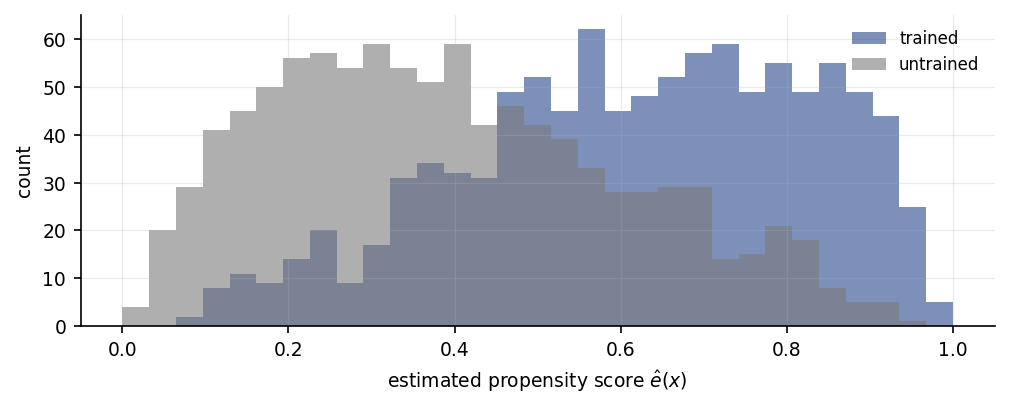
\includegraphics[width=0.72\textwidth,height=0.34\textheight,keepaspectratio]{cha10_propensity.png}
  \end{center}
  \begin{takeaway}[Check overlap before anything else]
    \footnotesize
    Matching needs treated and control units at \emph{comparable} scores. Where one
    histogram is empty, no method can compare --- those units have no counterpart.
  \end{takeaway}
\end{frame}

\begin{frame}{Propensity-score matching on the running example}
  {\footnotesize\textbf{Recipe (ATT):} for each treated unit, find the control with
  the nearest $\hat e(x)$ (with replacement); average the within-pair differences.}
  \begin{center}
    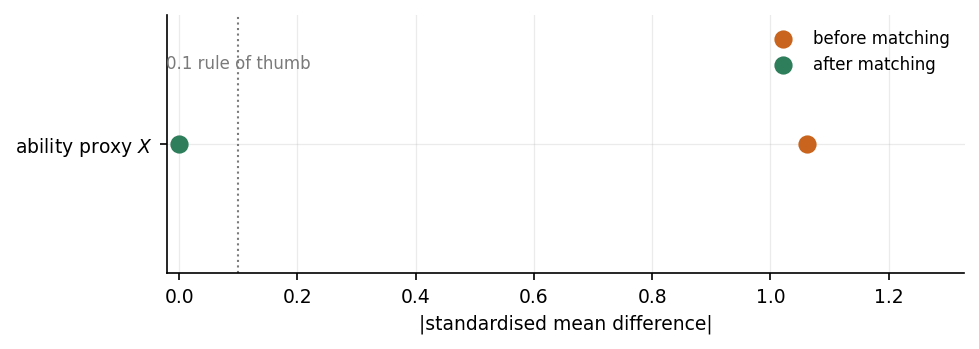
\includegraphics[width=0.62\textwidth,height=0.26\textheight,keepaspectratio]{cha10_balance.png}
  \end{center}
  \begin{numexample}[What matching bought us]
    \footnotesize
    Before matching the groups differ by $\mathbf{1.06}$ standard deviations on the
    ability proxy; after matching, $\mathbf{0.00}$. The estimate moves from the
    naive $2.53$ to $\mathbf{1.42}$ --- the same story as regression adjustment
    ($1.35$), because both lean on the same assumption.
  \end{numexample}
  \begin{mistake}
    Reporting the matched estimate without the balance picture --- the
    SMD-before/after plot \textbf{is} the evidence that matching did anything.
  \end{mistake}
\end{frame}

\begin{frame}{Adjustment scoreboard --- one simulation, four answers}
  \begin{center}
  \footnotesize
  \begin{tabular}{@{}lcl@{}}
    \toprule
    \textbf{Estimator} & \textbf{Estimate} & \textbf{Why it lands there} \\
    \midrule
    Truth (built into the simulation) & $1.00$ & --- \\
    Naive difference in means & $2.53$ & effect $+$ selection ($\gamma\delta$) \\
    Regression on $D$ and proxy $X$ & $1.35$ & removes measured confounding only \\
    Propensity matching on $X$ & $1.42$ & same assumption, same residual gap \\
    \bottomrule
  \end{tabular}
  \end{center}
  \begin{takeaway}[{{Adjustment methods agree with each other, not with the truth}}]
    Regression and matching answer the \emph{same} question two ways --- so their
    agreement is a consistency check, \textbf{not} a validation. Both still carry
    the confounding that the noisy proxy could not see.
  \end{takeaway}
\end{frame}

% ============================================================
\section{Difference-in-Differences}
% ============================================================

\begin{frame}{Using time as the control group}
  A policy hits one group (treated) and not another (control); you observe both
  \textbf{before} and \textbf{after}.
  \begin{block}{Rule}
    \[
      \boxed{\;\hat\tau_{\text{DiD}}
        = \big(\bar Y_{\text{T,after}} - \bar Y_{\text{T,before}}\big)
        - \big(\bar Y_{\text{C,after}} - \bar Y_{\text{C,before}}\big)\;}
    \]
  \end{block}
  \begin{readme}[How to read this]
    The control group's change estimates what would have happened to the treated
    \emph{anyway} (time trend, seasonality, the economy). Subtracting it removes any
    confounder that is \textbf{constant over time within group} --- even unmeasured
    ones. What it cannot remove: anything that changed for one group only.
  \end{readme}
\end{frame}

\begin{frame}{DiD in one picture}
  \begin{center}
    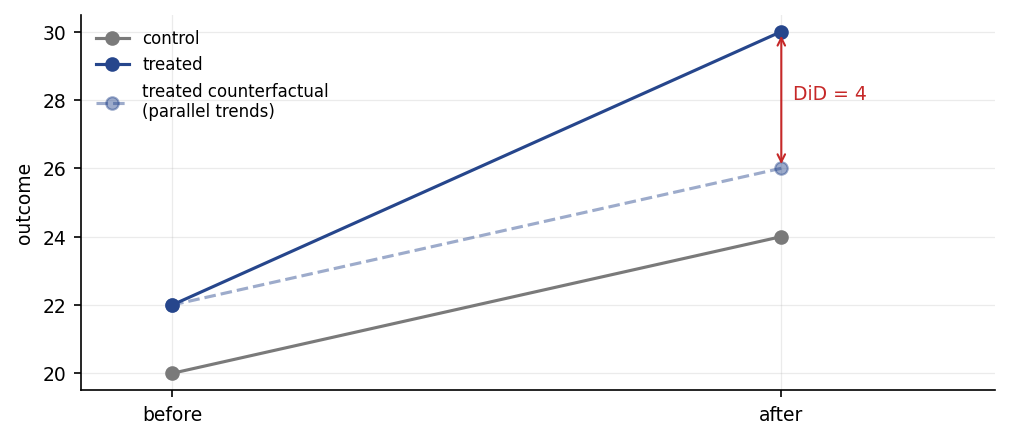
\includegraphics[width=0.74\textwidth,height=0.47\textheight,keepaspectratio]{cha10_did.png}
  \end{center}
  \begin{takeaway}[Parallel trends is the whole bet]
    \footnotesize
    Control rose $20 \to 24$; treated rose $22 \to 30$; DiD $= 8 - 4 = \mathbf{4}$.
    The dashed line is the assumption: untreated, the treated would have risen by
    the control's $+4$. Plot pre-period trends --- parallel \emph{before} is the
    only evidence you will ever get.
  \end{takeaway}
\end{frame}

\begin{frame}{Exercise A10.4 --- DiD by hand [Math]}
  \begin{exercise}
    A minimum-wage rise hits state T; neighbouring state C is untouched. Average
    monthly employment per fast-food store:
    \begin{center}
    \footnotesize
    \begin{tabular}{@{}lcc@{}}
      \toprule
      & \textbf{before} & \textbf{after} \\
      \midrule
      state T (treated) & $48$ & $60$ \\
      state C (control) & $50$ & $56$ \\
      \bottomrule
    \end{tabular}
    \end{center}
    \begin{enumerate}
      \item Compute the DiD estimate of the policy effect.
      \item Compute the two \emph{wrong} answers: after-minus-before for T only, and
            T-minus-C after only. What does each one confound the effect with?
      \item Name one concrete event that would break parallel trends here.
    \end{enumerate}
  \end{exercise}
\end{frame}

\begin{frame}{Solution --- Exercise A10.4}
  \begin{solutionbox}
    \footnotesize
    \textbf{Part 1.} $(60 - 48) - (56 - 50) = 12 - 6 = \mathbf{+6}$ jobs per store.
    \par\smallskip
    \textbf{Part 2.}
    \emph{Before-after in T only:} $+12$ --- confounds the policy with the common
    time trend (the economy grew: C rose $+6$ with no policy at all).
    \emph{T vs C after only:} $60 - 56 = +4$ --- confounds the policy with the
    \emph{permanent} level difference between the states (T started $2$ below C, so
    this understates).
    \par\smallskip
    \textbf{Part 3.} Any asymmetric shock: a factory opening in state T between the
    waves, a tourism collapse hitting only C's border towns, T announcing the rise
    early so stores hired ahead. Parallel trends is a claim about \emph{events},
    not about data.
  \end{solutionbox}
  \begin{mistake}
    Treating DiD as assumption-free because it ``differences everything out''. It
    differences out \emph{time-constant} confounding only --- the two wrong answers
    in part 2 are each one of the two things it removes.
  \end{mistake}
\end{frame}

% ============================================================
\section{Instrumental Variables}
% ============================================================

\begin{frame}{Borrowing someone else's randomness}
  When a confounder is unmeasured and untimed, one door remains: a variable $Z$ that
  \emph{nudges} treatment but has no path of its own to the outcome.
  \begin{center}
  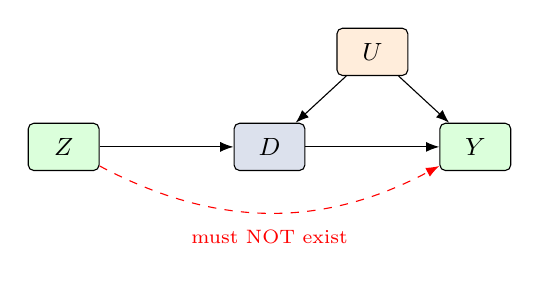
\begin{tikzpicture}[font=\small, node distance=1.1cm and 1.7cm,
      every node/.style={draw, rounded corners=2pt, minimum width=9mm, minimum height=6mm}]
    \node[fill=green!14] (Z) {$Z$};
    \node[right=of Z, fill=accent!16] (D) {$D$};
    \node[right=of D, fill=green!14] (Y) {$Y$};
    \node[above=9mm of $(D)!0.5!(Y)$, fill=orange!14] (U) {$U$};
    \draw[-{Latex}] (Z) -- (D);
    \draw[-{Latex}] (D) -- (Y);
    \draw[-{Latex}] (U) -- (D);
    \draw[-{Latex}] (U) -- (Y);
    \draw[-{Latex}, red, dashed] (Z) to[bend right=28] node[draw=none, below, red, font=\scriptsize]{must NOT exist} (Y);
  \end{tikzpicture}
  \end{center}
  \begin{block}{The three conditions}
    \begin{enumerate}
      \item \textbf{Relevance:} $Z$ actually moves $D$ (testable --- the first stage).
      \item \textbf{Exclusion:} $Z$ affects $Y$ \emph{only} through $D$ (not testable).
      \item \textbf{Independence:} $Z$ is as good as random --- unrelated to $U$
            (not testable).
    \end{enumerate}
  \end{block}
\end{frame}

\begin{frame}{The Wald estimator --- two small divisions}
  \begin{block}{Rule (binary $Z$)}
    \[
      \boxed{\;\hat\tau_{\text{IV}}
        = \frac{\bar Y_{Z=1} - \bar Y_{Z=0}}{\bar D_{Z=1} - \bar D_{Z=0}}\;}
      \qquad
      \frac{\text{effect of the nudge on the outcome}}{\text{effect of the nudge on take-up}}
    \]
  \end{block}
  \begin{readme}[How to read this]
    The numerator is an \emph{intention-to-treat} effect (module A1); the
    denominator is the \textbf{first stage}. Dividing scales the ITT up to the
    effect on those the nudge actually moved --- the \emph{compliers}. This is the
    same ITT logic A1 used for non-compliance, now run in reverse.
  \end{readme}
  \begin{numexample}[{{The running simulation, instrumented}}]
    A random encouragement $Z$ raises take-up by $0.40$ (first stage). Naive OLS:
    $\mathbf{2.33}$. Wald: $\mathbf{1.08}$ --- on top of the truth $1.0$, with the
    confounder $U$ still completely unobserved.
  \end{numexample}
\end{frame}

\begin{frame}{Three estimators, one target}
  \begin{center}
    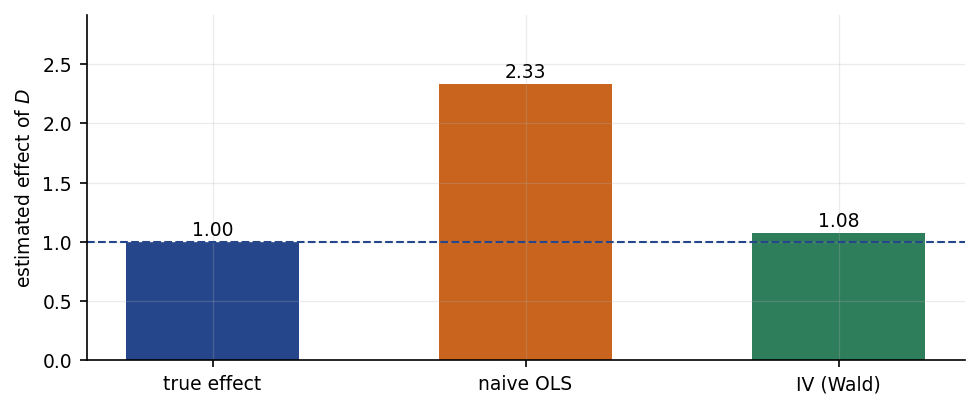
\includegraphics[width=0.66\textwidth,height=0.44\textheight,keepaspectratio]{cha10_iv.png}
  \end{center}
  \begin{takeaway}[Why IV wins here --- and what it costs]
    IV never observed the confounder, yet lands on the truth: the encouragement was
    \emph{randomised}, so its variation in $D$ carries no selection. The price:
    a \textbf{weak first stage} blows the variance up ($1/0.40$ scales every error),
    and the answer is the compliers' effect, not everyone's.
  \end{takeaway}
\end{frame}

\begin{frame}{Exercise A10.5 --- Is it an instrument? [Concept]}
  \begin{exercise}
    You want the effect of \textbf{university attendance} ($D$) on \textbf{earnings}
    ($Y$). For each candidate $Z$, check relevance / exclusion / independence and
    give a verdict:
    \begin{enumerate}
      \item \textbf{Distance to the nearest university} at age 18.
      \item \textbf{Parental education}.
      \item \textbf{A lottery} that randomly awards tuition waivers among applicants.
    \end{enumerate}
  \end{exercise}
\end{frame}

\begin{frame}{Solution --- Exercise A10.5}
  \begin{solutionbox}
    \footnotesize
    \textbf{Method.} Walk the three conditions; one clear failure kills the candidate.
    \begin{enumerate}
      \item \textbf{Distance:} relevance plausible (nearer $\Rightarrow$ more
            attendance --- check the first stage). Exclusion is the worry: families
            near universities differ (urban, richer labour markets pay differently).
            Verdict: \emph{usable only with controls for region --- and arguable}.
            This is the classic Card (1995) design and the classic objection to it.
      \item \textbf{Parental education:} relevant, yes --- but it fails
            independence/exclusion completely: it drives ability, networks and
            expectations, all of which touch earnings directly. Verdict:
            \emph{not an instrument; it is a confounder}.
      \item \textbf{The lottery:} relevance testable (waiver $\Rightarrow$ higher
            enrolment); independence holds by randomisation; exclusion plausible (a
            waiver moves earnings only via attendance --- unless the cash itself
            matters). Verdict: \emph{the best of the three by far}. Randomisation is
            what makes instruments credible --- which is why the strongest IVs are
            embedded experiments.
    \end{enumerate}
  \end{solutionbox}
\end{frame}

\begin{frame}{Reality check: Wage data}
  \begin{center}
    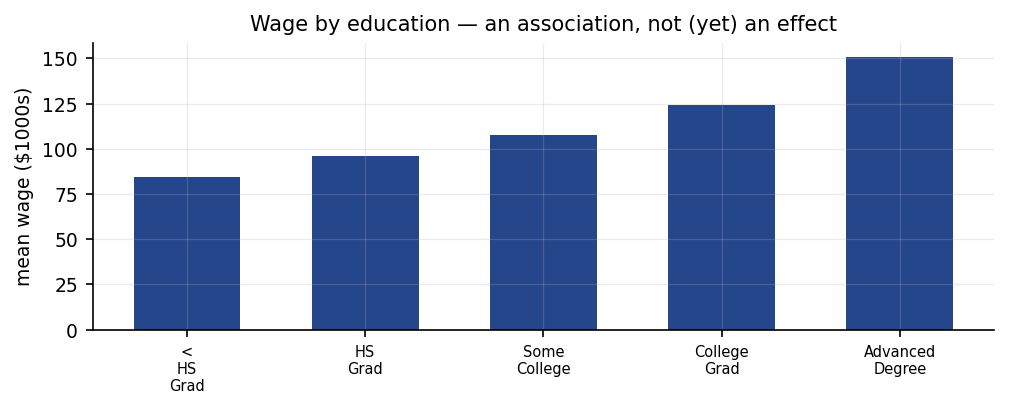
\includegraphics[width=0.74\textwidth,height=0.44\textheight,keepaspectratio]{cha10_wage_educ.png}
  \end{center}
  \begin{takeaway}[{{What we can, and cannot, say}}]
    College graduates out-earn non-graduates by $\mathbf{\$36.3}$k; adjusting for
    age and year barely moves it ($\$35.1$k). Nothing in this dataset measures
    ability or family background --- so this module's honest verdict is: a large,
    robust \emph{association}, whose causal share needs a design (a DiD, an
    instrument, a lottery) the data do not contain.
  \end{takeaway}
\end{frame}

\begin{frame}{Extended Exercise A10.1 --- Recover the truth in simulation [Python]}
  \begin{longexercise}
    Simulate the running example yourself ($n = 2000$, seed 2024):
    $U \sim N(0,1)$, $X = U + N(0, 0.5)$, $D = \mathbf{1}\{0.9U + N(0,1) > 0\}$,
    $Y = 2 + D + 1.5U + N(0,1)$.
    \begin{enumerate}
      \item Compute the naive difference in means and the regression-adjusted
            estimate (on $X$). Compare to $1.0$.
      \item Re-run with $X = U$ exactly (no proxy noise). What happens to the
            adjusted estimate, and why?
      \item Vary the proxy noise sd over $\{0, 0.25, 0.5, 1.0\}$ and plot the
            adjusted estimate against it. What does the curve tell you about
            ``controlling for'' badly measured confounders?
    \end{enumerate}
  \end{longexercise}
\end{frame}

\begin{frame}[fragile]{Solution --- Extended Exercise A10.1 (1/2)}
  \begin{solutionbox}[Solution --- code]
\begin{lstlisting}
import numpy as np
rng = np.random.default_rng(2024)
n, out = 2000, {}
for s in [0, 0.25, 0.5, 1.0]:          # proxy noise sd
    U = rng.normal(0, 1, n)
    X = U + rng.normal(0, s, n)
    D = (0.9*U + rng.normal(0, 1, n) > 0).astype(float)
    Y = 2 + D + 1.5*U + rng.normal(0, 1, n)
    naive = Y[D == 1].mean() - Y[D == 0].mean()
    Z = np.column_stack([np.ones(n), D, X])
    adj = np.linalg.lstsq(Z, Y, rcond=None)[0][1]
    out[s] = (naive, adj)
    print(f"noise sd {s}: naive {naive:.2f}, adjusted {adj:.2f}")
\end{lstlisting}
  \end{solutionbox}
\end{frame}

\begin{frame}{Solution --- Extended Exercise A10.1 (2/2)}
  \begin{solutionbox}[Solution --- reading the output]
    \footnotesize
    \textbf{Part 1.} With noise sd $0.5$ you reproduce the deck: naive
    $\approx 2.5$, adjusted $\approx 1.3$--$1.4$ (seed-dependent in the second
    decimal), truth $1.0$.
    \par\smallskip
    \textbf{Part 2.} With $X = U$ the adjusted estimate sits on $\approx 1.0$:
    unconfoundedness now holds \emph{exactly}, because the one confounder is fully
    observed. Adjustment works precisely when its assumption is true.
    \par\smallskip
    \textbf{Part 3.} The curve rises smoothly from $\approx 1.0$ (no noise) toward
    the naive value as the proxy degrades --- \textbf{measurement error in a
    confounder leaves residual confounding in proportion to the noise}. ``We
    controlled for income'' means little if income was self-reported in five broad
    bins.
  \end{solutionbox}
  \begin{mistake}
    Concluding from part 1 that adjustment ``does not work''. It did exactly what it
    promises: removed the bias carried by $X$. The shortfall is the part of $U$
    that $X$ never contained.
  \end{mistake}
\end{frame}

\begin{frame}{Extended Exercise A10.2 --- Design an observational study [Integrative]}
  \begin{longexercise}
    Your company rolled out a \textbf{sales-assistant AI} last year: teams could
    adopt it voluntarily, and adopters' revenue is now $18\%$ higher. The board
    asks: ``so it caused $18\%$?'' Design the honest analysis:
    \begin{enumerate}
      \item Name two plausible confounders and, for each, the \emph{sign} of the
            bias it induces (use $\gamma\delta$ reasoning).
      \item You have monthly revenue per team for two years. Which design from this
            module fits best, and what exactly would you compute?
      \item The rollout was staggered by region for logistics reasons unrelated to
            performance. What extra design does that enable?
      \item List the three robustness checks you would show the board.
    \end{enumerate}
  \end{longexercise}
\end{frame}

\begin{frame}{Solution --- Extended Exercise A10.2}
  \begin{solutionbox}
    \footnotesize
    \textbf{Part 1.} Team quality (good teams adopt tools \emph{and} sell more:
    $\gamma > 0, \delta > 0 \Rightarrow$ upward bias); desperation adoption
    (struggling teams grab tools: $\gamma < 0, \delta > 0 \Rightarrow$ downward
    bias). The $18\%$ could be either side of the truth.
    \par\smallskip
    \textbf{Part 2.} \textbf{Difference-in-differences} on the monthly panel:
    adopters vs never-adopters, change from the pre-adoption year to the
    post-adoption year --- with the pre-period trend plot as the parallel-trends
    evidence.
    \par\smallskip
    \textbf{Part 3.} The staggered, logistics-driven rollout is a candidate
    \textbf{instrument}: region-wave assignment shifts adoption timing (relevance,
    testable) and is plausibly unrelated to team quality (independence --- argue
    it). Compute the Wald ratio on early- vs late-wave regions.
    \par\smallskip
    \textbf{Part 4.} (i) Pre-trend plot; (ii) balance table on observables before/
    after matching; (iii) sensitivity: how strong an unmeasured confounder
    ($\gamma\delta$) would have to be to erase the estimate.
  \end{solutionbox}
\end{frame}

% ============================================================
\section{Python Lab}
% ============================================================

\begin{frame}{Python lab --- run it live}
  \begin{labnote}[{{Reproduce every number: \texttt{make\_figures.py}}}]
    Every estimate quoted on these slides is computed by
    \texttt{make\_figures.py} in this module's folder, from seeded simulations and
    the bundled \texttt{Wage.csv} --- run it and read it alongside the deck:
    \begin{itemize}
      \item the running simulation: naive $2.53$ / adjusted $1.35$ / matched $1.42$;
      \item the from-scratch logistic propensity model and 1:1 matching (ATT);
      \item the DiD figure and the IV simulation (OLS $2.33$ vs Wald $1.08$);
      \item the \texttt{Wage} education gaps ($36.3$ naive, $35.1$ adjusted).
    \end{itemize}
    A companion notebook in the course lab format is in preparation; until it
    lands, the script \emph{is} the lab --- it runs top to bottom in the course
    environment with no extra packages.
  \end{labnote}
\end{frame}

\begin{frame}[fragile]{The whole module in fifteen lines}
\begin{lstlisting}
import numpy as np
rng = np.random.default_rng(2024)
n = 2000
U = rng.normal(0, 1, n)                    # unmeasured ability
X = U + rng.normal(0, 0.5, n)              # what we actually observe
D = (0.9*U + rng.normal(0, 1, n) > 0).astype(float)
Y = 2 + 1.0*D + 1.5*U + rng.normal(0, 1, n)

naive = Y[D == 1].mean() - Y[D == 0].mean()          # 2.53
Z = np.column_stack([np.ones(n), D, X])
adjusted = np.linalg.lstsq(Z, Y, rcond=None)[0][1]   # 1.35

print(f"truth 1.00 | naive {naive:.2f} | adjusted {adjusted:.2f}")
# adjustment removes the bias carried by X -- and only that
\end{lstlisting}
\end{frame}

% ============================================================
\section{Summary}
% ============================================================

\begin{frame}{Module A10 in one slide}
  \begin{block}{What we accomplished}
    Four honest ways to chase a causal effect when nobody randomised --- each with
    its assumption stated out loud.
  \end{block}
  \begin{itemize}
    \item Naive comparison $=$ effect $+$ selection: on our simulation, $2.53$
          for a true $1.0$.
    \item Omitted-variable bias $= \gamma\,\delta$: sign and size it without data.
    \item Adjust / stratify / match on observables: $2.53 \to 1.35$--$1.42$ ---
          exactly as far as the measured $X$ reaches, never further.
    \item Difference-in-differences: time-constant confounding cancels; parallel
          trends is the bet.
    \item Instrumental variables: the Wald ratio $1.08$ recovers the truth without
          ever seeing $U$ --- if the instrument is truly excludable.
  \end{itemize}
\end{frame}

\begin{frame}{Key formulas at a glance}
  \footnotesize
  \begin{description}
    \item[Omitted-variable bias] short $= \tau + \gamma\delta$, with
      $U = \delta_0 + \delta D + v$.
    \item[Unconfoundedness] $\{Y(1), Y(0)\} \perp D \mid X$ --- the licence for all
      adjustment methods.
    \item[Propensity score] $e(x) = \Pr(D=1 \mid X=x)$; balance on $e(X)$ suffices.
    \item[SMD balance check] $(\bar x_1 - \bar x_0)\big/\sqrt{(s_1^2 + s_0^2)/2}$;
      aim below $0.1$.
    \item[DiD] $(\bar Y_{T,\text{aft}} - \bar Y_{T,\text{bef}}) -
      (\bar Y_{C,\text{aft}} - \bar Y_{C,\text{bef}})$.
    \item[Wald / IV] $(\bar Y_{Z=1} - \bar Y_{Z=0}) \big/
      (\bar D_{Z=1} - \bar D_{Z=0})$ --- ITT scaled by the first stage.
  \end{description}
\end{frame}

\begin{frame}{Vocabulary checklist}
  \footnotesize
  \begin{center}
  \begin{tabular}{@{}ll@{}}
    \toprule
    \textbf{Term} & \textbf{Meaning} \\
    \midrule
    confounder & common cause of $D$ and $Y$; adjust for it \\
    mediator & lies on the causal path; do not adjust \\
    collider & common \emph{effect}; adjusting creates bias \\
    unconfoundedness & all confounders measured --- untestable licence to adjust \\
    propensity score & $\Pr(D=1\mid X)$; one scalar summarising all covariates \\
    overlap / common support & both groups present at every propensity value \\
    parallel trends & DiD's assumption: equal untreated time-paths \\
    instrument & shifts $D$; touches $Y$ only through $D$; as-good-as-random \\
    first stage & effect of $Z$ on $D$; weak $\Rightarrow$ unstable IV \\
    complier & unit whose $D$ the instrument actually moves \\
    \bottomrule
  \end{tabular}
  \end{center}
\end{frame}

\begin{frame}{Decision rules of thumb}
  \begin{itemize}
    \item Randomised? Use module A1 and stop. Observational? Start from the diagram,
          not from the regression.
    \item Adjust for confounders only --- never mediators, never colliders, never
          post-treatment variables of any kind.
    \item Before matching or weighting: plot propensity \textbf{overlap}. After:
          show the \textbf{balance} table. No overlap $\Rightarrow$ no comparison.
    \item Panel data and a clean untreated group $\Rightarrow$ prefer DiD; always
          plot pre-trends.
    \item An instrument beats adjustment \emph{only if} you can argue exclusion out
          loud; check the first stage before trusting anything.
    \item Whatever you estimate, attach the sensitivity question: how big a
          $\gamma\delta$ would undo it?
  \end{itemize}
\end{frame}

\begin{frame}{Common pitfalls}
  \begin{alertblock}{Don't}
    \begin{enumerate}
      \item Read a regression coefficient on observational data as an effect
            because the $p$-value is small.
      \item Control for everything the dataset offers (mediators and colliders
            included).
      \item Match without checking overlap and balance --- or report the estimate
            without them.
      \item Run DiD without a pre-trend plot.
      \item Use a clever instrument with a first stage of $0.05$.
      \item Forget that adjustment on a noisy proxy leaves bias in proportion to
            the noise.
    \end{enumerate}
  \end{alertblock}
\end{frame}

\begin{frame}{Self-check questions}
  \scriptsize
  \begin{readme}[{{Quick self-assessment}}]
    \begin{enumerate}
      \item The naive gap is $2.53$ and the truth $1.0$. Which two numbers multiply
            to the bias, and what are they called?
      \item Tar deposits in the smoking--disease study: adjust or not, and why?
      \item Treated: low $5.0$ ($n{=}20$), high $9.0$ ($n{=}80$); control: low $4.0$
            ($n{=}80$), high $8.0$ ($n{=}20$). Naive and stratified estimates?
      \item Control $50 \to 56$, treated $48 \to 60$: the DiD estimate, and the
            assumption it rests on?
      \item Wald: ITT $= 0.43$, first stage $= 0.40$. The IV estimate --- and whose
            effect is it?
      \item Matching moved the SMD from $1.06$ to $0.00$ yet the estimate is still
            $1.42$, not $1.0$. What explains the gap?
    \end{enumerate}
  \end{readme}
  \begin{takeaway}[{{Answers}}]
    (1) $\gamma$ (confounder $\to$ outcome) $\times$ $\delta$ (group gap in the
    confounder) --- omitted-variable bias. (2) Do not adjust: it is a mediator; you
    would delete the effect's pathway. (3) Naive $8.2 - 4.8 = 3.4$; stratified
    $1.0$. (4) $12 - 6 = 6$; parallel trends. (5) $0.43/0.40 \approx 1.08$; the
    compliers'. (6) $X$ is a noisy proxy --- balance on $X$ is not balance on $U$;
    residual confounding remains.
  \end{takeaway}
\end{frame}

\begin{frame}{Five things to remember}
  \begin{takeaway}[Module A10 in five lines]
    \begin{enumerate}
      \item \textbf{No design, no effect.} A coefficient is causal because of an
            argument about the world, never because of a fit statistic.
      \item \textbf{Bias $= \gamma\,\delta$.} Two numbers you can reason about even
            when you cannot measure them.
      \item \textbf{Adjustment reaches exactly as far as your covariates} --- our
            noisy proxy took $2.53$ to $1.4$, not to $1.0$.
      \item \textbf{DiD trades confounders for one assumption} --- parallel trends
            --- and pre-trends are the only evidence for it.
      \item \textbf{An instrument imports randomisation}: Wald $= $ ITT / first
            stage landed on $1.08$ without ever seeing the confounder.
    \end{enumerate}
  \end{takeaway}
\end{frame}

\begin{frame}{What's next}
  \begin{itemize}
    \item \textbf{Module A1 --- Randomised Controlled Trials} is this module's
          prerequisite and its benchmark: every method here is an attempt to
          reconstruct, by argument, what randomisation buys by design.
    \item \textbf{Module A2 --- Explainable AI with Shapley Values}: its Pitfall 2
          (``an explanation is not a cause'') is precisely this module's subject ---
          now you have the vocabulary to say why.
    \item \textbf{Module A7 --- Multiple Testing}: subgroup-hunting for the segment
          where the effect ``works'' is a multiplicity problem before it is a causal
          one.
  \end{itemize}
\end{frame}

% ============================================================
\appendix
\AtBeginSection[]{}
\section{Appendix: optional and advanced material}
% ============================================================

\begin{frame}{Appendix --- what is in here, and why}
  \footnotesize
  Nothing in the appendix is needed to follow the module: each slide is a formal
  derivation, a longer worked exercise, or a side topic. Read it when you want the
  full story, or when a later chapter sends you back here.
  \begin{block}{Contents of the appendix}
    \begin{itemize}
      \item \textbf{Deriving the OVB formula} --- three lines of Chapter 3 algebra;
            moved out because the result, not the derivation, is what the module
            uses.
      \item \textbf{ATT vs ATE} --- which average the estimators actually target;
            moved out because the distinction matters only once the main ideas sit.
      \item \textbf{Two-stage least squares} --- the regression form of the Wald
            estimator, for continuous instruments and controls.
    \end{itemize}
  \end{block}
\end{frame}

\begin{frame}{Deriving the omitted-variable-bias formula}
  \footnotesize
  Long model: $Y = \beta_0 + \tau D + \gamma U + \varepsilon$; auxiliary:
  $U = \delta_0 + \delta D + v$ with $v \perp D$ by construction. Substitute:
  \[
    Y = \beta_0 + \tau D + \gamma(\delta_0 + \delta D + v) + \varepsilon
      = \underbrace{(\beta_0 + \gamma\delta_0)}_{\text{new intercept}}
        + \underbrace{(\tau + \gamma\delta)}_{\text{short-regression slope}} D
        + \underbrace{(\gamma v + \varepsilon)}_{\text{error, } \perp D}.
  \]
  The composite error is uncorrelated with $D$, so OLS on $D$ alone estimates
  $\tau + \gamma\delta$ consistently --- consistently \emph{wrong}, by exactly the
  bias term.
  \begin{takeaway}[Why this is worth three lines]
    Every ``controlling for X changed my coefficient'' moment in Chapter 3 is this
    identity in motion. It also powers sensitivity analysis: solve
    $\gamma\delta = \hat\tau_{\text{naive}} - 0$ to find how strong a confounder
    must be to explain your whole estimate.
  \end{takeaway}
\end{frame}

\begin{frame}{ATT, ATE, and what each estimator targets}
  \footnotesize
  \begin{center}
  \begin{tabular}{@{}lll@{}}
    \toprule
    \textbf{Estimand} & \textbf{Question} & \textbf{Natural estimator} \\
    \midrule
    ATE $= E[Y(1) - Y(0)]$ & effect for a random unit & stratification weighted by
    stratum size \\
    ATT $= E[Y(1) - Y(0) \mid D = 1]$ & effect for those treated & matching treated
    to controls \\
    LATE & effect for compliers & Wald / IV \\
    \bottomrule
  \end{tabular}
  \end{center}
  \begin{readme}[Why the distinction matters]
    Under treatment-effect \emph{heterogeneity} these differ. Our matching estimator
    reproduced each treated unit's counterfactual --- an ATT. The IV answered for
    compliers only --- a LATE. Neither is wrong; each answers a different policy
    question (``should we keep the programme for its users?'' vs ``what if we
    enrolled everyone?'').
  \end{readme}
\end{frame}

\begin{frame}{Two-stage least squares (2SLS)}
  \footnotesize
  \begin{block}{Algorithm}
    \begin{enumerate}
      \item \textbf{First stage:} regress $D$ on $Z$ (and controls $X$); keep
            fitted $\hat D$.
      \item \textbf{Second stage:} regress $Y$ on $\hat D$ (and the same $X$); the
            coefficient of $\hat D$ is $\hat\tau_{\text{2SLS}}$.
    \end{enumerate}
  \end{block}
  \begin{readme}[How to read this]
    $\hat D$ keeps only the part of treatment variation that the instrument
    explains --- the part with no selection in it. With one binary $Z$, no controls,
    2SLS \emph{equals} the Wald ratio exactly. Report the first-stage $F$: below
    $\sim 10$, the instrument is too weak to trust (our simulation's first stage of
    $0.40$ on $n = 5000$ is comfortably strong).
  \end{readme}
  \begin{mistake}
    Running the two stages by hand and using the second stage's printed standard
    errors --- they ignore that $\hat D$ was estimated. Real implementations
    (\texttt{linearmodels.IV2SLS}) correct this.
  \end{mistake}
\end{frame}

\end{document}
